\capitulo{3}{Conceptos teóricos}

A continuación se explicaran algunos conceptos teóricos tanto de la parte técnica como de la parte de procesos de software.


\section{Deuda técnica}

La metáfora de deuda nació como una forma de expresar la diferencia entre el entendimiento del programa (la abstracción) y su implementación \cite{cu09}.

Con el tiempo surgió un término similar; la deuda técnica, que es la metáfora que expresa el coste que conlleva el dejar código que no tiene un buen diseño en el proyecto. Si seguimos manteniendo el proyecto, esta deuda cada vez costará más el arreglarla y tendremos que pagar los intereses \cite{fow03}.

Las razones de incremento de la deuda con el paso del tiempo pueden ser el simple hecho de olvidar cómo funciona cada línea de código, o la complejidad emergente del acoplamiento de código antiguo con otro nuevo sin cambiar las abstracciones ni desacoplar el código.

\begin{figure}
	\centering
	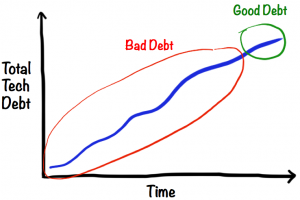
\includegraphics[width=0.8\textwidth]{deuda1.png}
	\caption[Deuda técnica: Beneficiosa y perjudicial]{Deuda técnica: Beneficiosa y perjudicial\cite{kni13}.}\label{fig:deuda1.png}
\end{figure}


Este tipo de deuda se ve como necesaria, según algunos autores \cite{kni13}, se debe incurrir en deuda técnica, ya que es beneficioso para el desarrollo. Esto se debe a que, a corto plazo, es imposible prever cómo se va a desarrollar el proyecto, y unos cambios demasiado tempranos, pueden ser un mal diseño a medio o largo plazo. La deuda `buena' o beneficiosa se suele considerar como aquella que como mucho dura una semana, una vez existe por más tiempo pasa a ser cada vez más costosa de solucionar o `pagar'.


Una característica importante de esta deuda es que una vez dejas de soportar el mantenimiento de un proyecto, la deuda técnica desaparece, al contrario que la deuda financiera.

Se puede idealizar la deuda técnica y considerar que todas las semanas en las que se dedica una cantidad de tiempo a solucionarla esta deuda técnica desaparece, pero esto no corresponde con la realidad. Normalmente, la deuda, aunque se solucione, suele ir incrementando poco a poco, debido a la complejidad de un sistema mantenido a lo largo de una gran cantidad de tiempo.

La manera de tener esto en cuenta es tener un `techo de deuda'. Este techo debería ser lo suficientemente alto como para que no se alcance todos los meses, pero no demasiado alto como para que cuando se llegue al techo fijado, el proyecto sea directamente un fracaso o demasiado caro de pagar.

La opinión de algunas personas es que se debe llegar al techo cada 6 meses, desde mi propia inexperiencia, creo que deberíamos evaluar la deuda a los 4 meses, para ver si la re-estructuración del proyecto es viable e intentar buscar un punto de tiempo en el que el pagar la deuda técnica sea algo más simple, ya que si esperamos hasta los 6 meses, probablemente no podamos elegir un momento óptimo. 

\begin{figure}
	\centering
	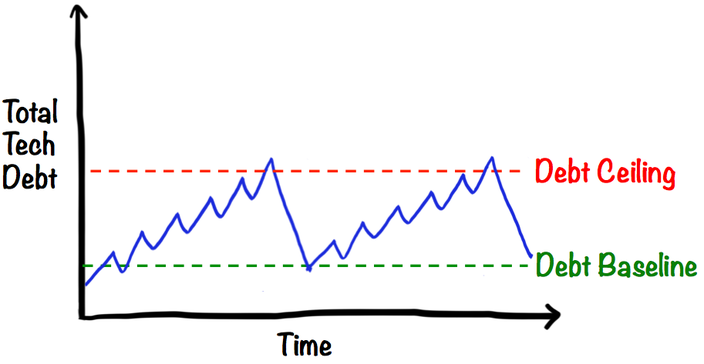
\includegraphics[width=0.8\textwidth]{deuda2.png}
	\caption{Deuda técnica: Techo y base \cite{kni13}}\label{fig:deuda2.png}
\end{figure}

Es importante destacar que existen otros argumentos para mantener la deuda técnica baja, al que menos importancia parece darse es que la deuda técnica es algo difícilmente cuantificable hasta que se refactoriza, si no la reducimos, no sabemos cuanta tenemos.

\FloatBarrier

\section{Integración continua (\textit{Continuous Integration})}

Acortado con las siglas CI, es un método habitual para reducir la deuda técnica. Es la práctica de ejecutar y testear conjuntamente todos los servicios que deban ir relacionados una vez se inicie el despliegue en producción. Esto nos asegura que van a funcionar en producción la mayoría de las veces, unas pocas veces habrá problemas por la escalabilidad, errores dado el cambio del hardware, problemas con el rendimiento... Un ejemplo es si ejecutamos Java y los test no fallan, pero al ponerlo en producción le damos a la JVM más de 200 GB de memoria RAM, esto causa comportamientos inesperados.

\subsection{Entrega continua (\eng{Continuous Delivery})}

Es un término asociado a CI, consiste en un proyecto que dispone de CI y buena cantidad de test de calidad, una vez ya tengamos un sistema a punto podemos empezar a modificar o mejorar funcionalidades añadiéndolas directamente a producción si pasa los test, requiere que hagamos los test casi a la vez que el código. Esto fomenta y premia técnicas como \eng{extreme programming} (XP) que se basan en TDD (\eng{Test Driven Development}), una forma de programar que pide que hagamos los test antes que el resto del código.


\section{DevOps}

\eng{DevOps} es un acrónimo inglés de: `\eng{software \textbf{Dev}elopment and information technology \textbf{Op}eration\textbf{s}}' es un término que engloba un conjunto de prácticas de colaboración y comunicación entre desarrolladores software y técnicos informáticos. Los objetivos de esta comunicación y colaboración son una construcción de software más consistente y confiable. Este proceso, heredero de las técnicas ágiles, se basa en una \textit{cadena de herramientas}. Esta cadena de herramientas es algo que no está completamente definido, pero más o menos la podemos concretar. Cabe tener en cuenta que esta cadena cambia según a quien le preguntes.

\subsection{La `\emph{cadena de herramientas}' de DevOps}

Esta cadena de herramientas se basa en siete procesos con sus correspondientes herramientas:

\begin{enumerate}
 \item \textbf{Plan}: Consistente en determinación de métricas, requerimientos... y una vez pasemos de la primera iteración ha de tener en cuenta el feedback del cliente.
 \item \textbf{Creación}: Es el proceso de programar y crear el software, la herramienta en este proceso es el software de control de versiones que vayamos a usar.
 \item \textbf{Verificación}: Proceso de comprobación de la calidad del software. Normalmente consiste en hacer test de diversos tipos (aceptación, seguridad...)
 \item \textbf{Preproducción} o \textbf{empaquetación}: En esta fase se piden aprobaciones de los distintos equipos y se configura el paquete.
 \item \textbf{Lanzamiento}: En este punto se prepara el horario de lanzamiento y se orquesta el software para poder desplegarlo en el entorno de producción objetivo.
 \item \textbf{Configuración}: Una vez el software está desplegado toda la parte de la infraestructura y configuración de la misma se incluye en esta categoría, como por ejemplo las bases de datos, configuración de las mismas...
 \item \textbf{Monitorización}: Tras entregar el software, se mide su rendimiento en la infraestructura objetivo y se mide la satisfacción del usuario final. Se recogen métricas y estadísticas
\end{enumerate}


\section{Microservicios}

Los microservicios son una arquitectura y un patrón de diseño, que no se ha inventado en un momento concreto, si no que ha surgido como una tendencia o patrón del diseño de sistemas en el mundo real. 

Un microservicio es un servicio pequeño y autónomo que puede trabajar junto a otros, es importante que tenga un objetivo claro y que lo haga bien.

Esto está reforzado por el concepto del «\emph{Principio de responsabilidad única}» de C. Martin\cite{martin03} «\emph{Juntar aquellas cosas que cambian por la misma razón y separar aquellas que cambian por razones diferentes}».

El tamaño de un microservicio es algo muy discutido, pero generalmente se requiere que sea mantenible por un equipo `pequeño' (6-10 personas), y se pueda reescribir en 2 semanas.

Esto se debe conseguir mediante una interfaz de programación de aplicación (API: \eng{Application Programming Interface}), que permita a los clientes acceder al servicio sin causar acoplamiento, algo más difícil de hacer que de decir.

Los principales beneficios son:
\begin{itemize}
\item \textbf{Sistemas heterogéneos}: Facilita usar distintas tecnologías en distintos sistemas, para usar la mejor herramienta en cada ocasión.
\item \textbf{Resiliencia}: Si falla un microservicio, el resto del sistema se puede mantener levantado, aislando los problemas y facilitando la alta disponibilidad.
\item \textbf{Escalabilidad}: En caso de que una parte del sistema necesite mayor número de recursos, podemos crear una nueva instancia sin cambiar el funcionamiento del resto del sistema.
\item \textbf{Facilidad de despliegue}: Los cambios se mantienen más contenidos, permitiendo cambiar solo un microservicio por su versión actualizada y no todo el sistema.
\item \textbf{Replazabilidad}: Un microservicio que pasa a ser obsoleto, puede ser reemplazado o eliminado, en vez de tener que mantenerlo porque al eliminarlo se rompe todo el sistema, algo que no debería pasar, pero que es común en los sistemas legados.
\item \textbf{Test a nivel de servicio}: Cada microservicio se puede testear por cuenta propia, de manera que aunque el sistema aumenten su complejidad, podamos controlar cada microservicio por separado.
\end{itemize}

\begin{figure}
	\centering
	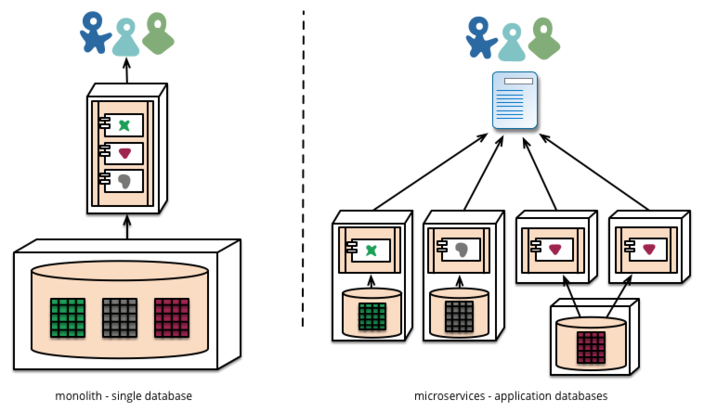
\includegraphics[width=0.8\textwidth]{microvsmono.png}
	\caption[Arquitecturas monolítica y microservicios]{Arquitecturas monolítica y microservicios.\cite{fow14}.}\label{fig:microvsmono.png}
\end{figure}

Estos beneficios por supuesto vienen con desventajas:

\begin{itemize}
\item \textbf{Distribución}: Raramente se van a ver microservicios en una arquitectura que no esté distribuida, esto hace que sea más difícil de programar y tengamos que tener en cuenta otros errores.
\item \textbf{Seguridad}: Es más difícil asegurar la seguridad de un microservicio, ya que debemos protegernos contra más puntos de vulnerabilidad, a no ser que estemos ejecutando en un clúster seguro.
\item \textbf{Complejidad de operación}: Hace falta un equipo de operaciones con madurez, de manera que se puedan redistribuir los microsistemas regularmente.
\item \textbf{Test a nivel de sistema}: Los test a nivel de sistema incrementan algo su complejidad, ya que vamos a tener que usar microservicios falsos, como mocks o similares casi siempre, a no ser que estemos en un sistema pequeño.
\end{itemize}

Por último, vale la pena hablar del coste en productividad, esto no es una ventaja ni un perjuicio, es un \textit{trade-off}, un intercambio.

En un sistema monolítico, tenemos menos coste en productividad, hasta que llegamos a un punto crítico en el que la complejidad aumenta demasiado o necesitamos escalar.

En los microservicios, tenemos menos coste a la hora de seguir iterando, aumentando la complejidad de un sistema, pero a cambio tenemos mayor barrera de entrada, hasta que se tiene el primer prototipo funcional. Además los desarrolladores tienen que aprender cómo programar bajo esta arquitectura.

\section{Deep Learning}

Definido estrictamente el \eng{deep learning} consiste en el uso de redes neuronales artificiales con más de una capa oculta. 

\subsection{Redes neuronales artificiales}

Las redes neuronales son sistemas de computación inspirados por las redes neuronales biológicas, que podemos encontrar en los cerebros de los animales. Estos sistemas requieren un tiempo de `aprendizaje' (entrenamiento o mejora progresiva del rendimiento) para, a partir de unos ejemplos, resolver una tarea.

Hoy en día, las redes neuronales artificiales se forman a partir de un grafo acíclico dirigido, y se organizan típicamente en capas. Las capas más comunes son: 
\begin{itemize}
\item \textbf{La capa de entrada}: donde la red recibe los datos.
\item \textbf{Las capas ocultas}: que son las que `aprenden' mediante ajustes a sus propiedades.
\item \textbf{La capa de salida}: que devuelve la predicción o resultado deseado.
\end{itemize}

Las propiedades que tienen las capas intermedias son:

\begin{itemize}
\item \textbf{La función de activación}: esta es la función que determina si la neurona se activa (pasa información a otras neuronas) o no. En algunos modelos siempre pasan información y esta función simplemente la modifica. Las más usadas son: 
\item \textbf{Los pesos}: son la parte que cambia al entrenar el modelo, de manera que afectará al resultado.
\end{itemize}

La forma de cambiar los pesos y de que la red aprenda se llama propagación hacia atrás (\eng{backprop} o \eng{backpropagation}), que calcula el gradiente de la función de perdida (diferencia entre el valor y el objetivo). 

\subsection{Redes neuronales convolucionales}
Las redes neuronales convolucionales se distinguen de las redes neuronales tradicionales en las capas que las componen, capas convolucionales.

La convolución es una operación matemática diseñada para imitar el estimulo producido en una neurona de la corteza cerebral en respuesta a una imagen.


\begin{figure}
	\centering
	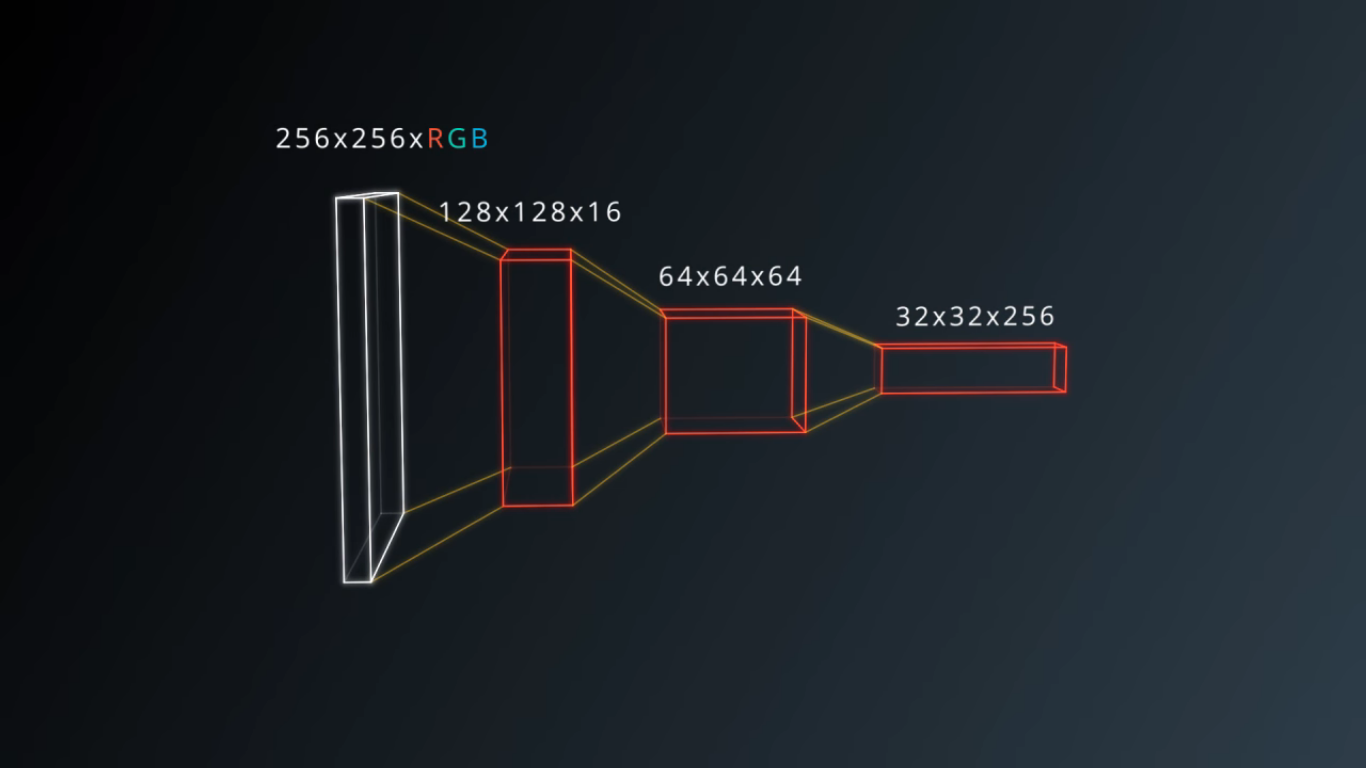
\includegraphics[width=0.8\textwidth]{CNN.png}
	\caption[Red neuronal convolucional]{Red neuronal convolucional: imagen de \href{https://www.udacity.com/course/deep-learning--ud730}{Udacity: https://www.udacity.com/course/deep-learning--ud730}}\label{fig:CNN.png}
\end{figure}
\FloatBarrier
La potencia de la convolución se presenta a la hora de pasar una ventana por distintas partes de la entrada con los mismos pesos, aprendiendo así patrones más complejos.

La primera red neuronal convolucional ampliamente reconocida es LeNet-5 por Yann LeCunn \cite{lecun98}. 

A partir de esta se desarrollan otras, como por ejemplo, AlexNet\cite{alexnet} e \eng{inception}\cite{incep}.

En este trabajo se presenta el uso y re-entrenamiento de \eng{inception} v3.

\begin{figure}
	\centering
	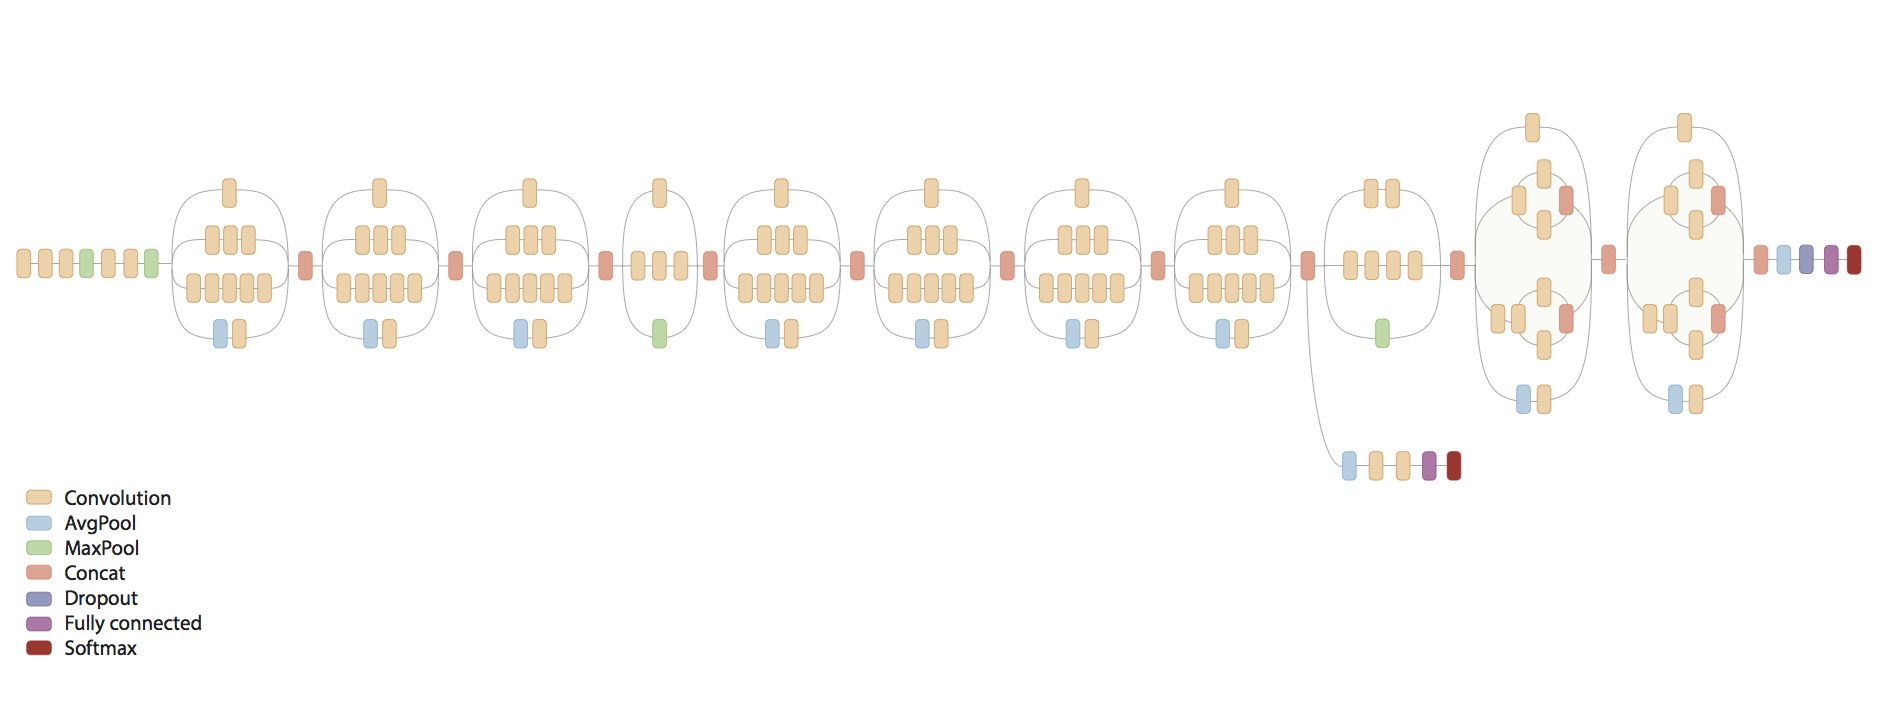
\includegraphics[width=0.8\textwidth]{incep_arch.png}
	\caption[Arquitectura inception v3]{Arquitectura inception v3: imagen de \href{https://github.com/tensorflow/models/tree/master/inception}{Tensorflow: https://github.com/tensorflow/models/tree/master/inception}}\label{fig:incep_arch.png}
\end{figure}
\FloatBarrier
Cabe destacar que \eng{inception} presenta una diferencia importante respecto a las arquitecturas anteriores, en vez de elegir entre una convolución 1x1, 3x3, 5x5 o un \eng{pooling}\footnote{\eng{Pooling}: operación que consiste en devolver el valor más alto/medio/más bajo de la ventana a la que se aplica.}, los módulos \eng{inception} hacen todas las operaciones y las combinan en el resultado.

\begin{figure}
	\centering
	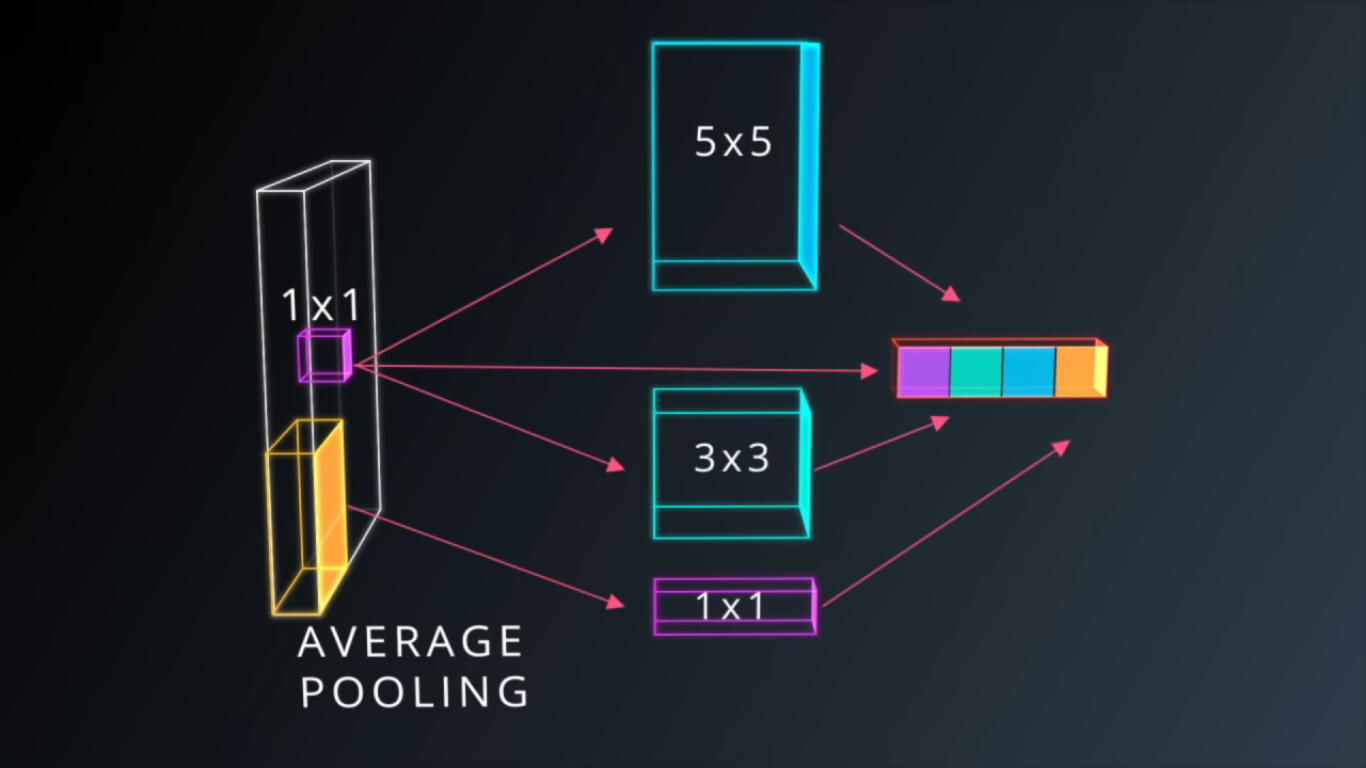
\includegraphics[width=0.8\textwidth]{incep_module.png}
	\caption[Módulo inception]{Modulo inception: imagen de \href{https://www.udacity.com/course/deep-learning--ud730}{Udacity: https://www.udacity.com/course/deep-learning--ud730}}\label{fig:incep_module.png}
\end{figure}









